\documentclass[10pt, aspectratio=169, handout]{beamer}
\usefonttheme{professionalfonts}

\mode<presentation>
{ 
  \usetheme{Berkeley}
  \usecolortheme{beaver}
  \usefonttheme{default}
  \setbeamertemplate{navigation symbols}{} 
  \setbeamertemplate{caption}[numbered]
} 

\setbeamertemplate{footline}{%
  \leavevmode%
  \hbox{% 
    \begin{beamercolorbox}[wd=.85\paperwidth,ht=2.5ex,dp=1ex,left]{author in head/foot}% 
      \usebeamerfont{author in head/foot}Digital Signal Processing, Fall 2025%
    \end{beamercolorbox}% 
    \begin{beamercolorbox}[wd=.15\paperwidth,ht=2.5ex,dp=1ex,right]{date in head/foot}% 
      \hspace*{0.5em}\insertframenumber{} / \inserttotalframenumber\hspace*{0.5em}% 
    \end{beamercolorbox}% 
  }%
  \vskip0pt%
}

\usepackage[english]{babel}
\usepackage[utf8x]{inputenc}
\usepackage{tikz}
\usepackage{pgfplots}
\usepackage{array}
\usepackage{makecell}
\usepackage{verbatim}
\usepackage{graphicx}
\usepackage{subcaption}
\usepackage{amsfonts}
\usepackage{amsmath}
\usepackage{bm}
\usepackage{epstopdf}
\captionsetup{compatibility=false}
\usepackage[absolute,overlay]{textpos}
\usetikzlibrary{calc}
\usetikzlibrary{pgfplots.fillbetween, backgrounds}
\usetikzlibrary{positioning}
\usetikzlibrary{pgfplots.groupplots}
\usetikzlibrary{plotmarks}
\usetikzlibrary{calc}
\usepgfplotslibrary{groupplots}
\pgfplotsset{compat=newest} 

\usepackage{hyperref}
\hypersetup{
    colorlinks=true,
    linkcolor=blue,
    filecolor=magenta,      
    urlcolor=cyan,
}

\title[ECEN 463/863]{Sampling of Continuous-Time Signals}
\author{Department of Electrical and Computer Engineering}
\institute{University of Nebraska-Lincoln}
\date{Fall 2025}

\begin{document}

\begin{frame}
  \titlepage
\end{frame}

\section{Introduction}

\begin{frame}{Periodic Sampling: Basic Definition}
\textbf{Fundamental Sampling Equation}:
\[
x[n] = x_c(nT), \quad -\infty < n < \infty
\]

\vspace{0.3cm}
\textbf{Key Parameters}:
\begin{itemize}
    \item $T$ = Sampling period (seconds)
    \item $f_s = \frac{1}{T}$ = Sampling frequency (samples/second or Hz)
    \item $\Omega_s = \frac{2\pi}{T}$ = Sampling frequency (radians/second)
\end{itemize}

\vspace{0.3cm}
\textbf{Ideal C/D Converter}:
\begin{center}
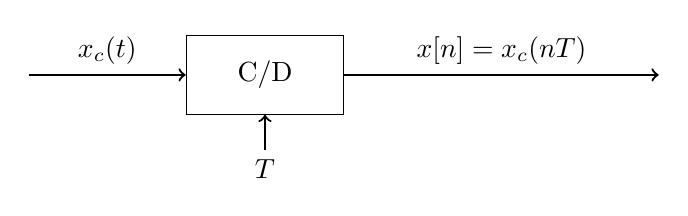
\begin{tikzpicture}
    % C/D box at (-2,0)
    \node[draw, minimum width=2cm, minimum height=1cm] (cd) at (-2,0) {C/D};
    % Input arrow: from far left to left side of box
    \draw[->, thick] (-5,0) -- (cd.west) node[midway, above] {$x_c(t)$};
    % Output arrow: from right side of box to far right
    \draw[->, thick] (cd.east) -- (3,0) node[midway, above] {$x[n] = x_c(nT)$};
    % T node below box
    \node (Tlabel) at (-2,-1.2) {$T$};
    % Arrow from T label into bottom of box
    \draw[->, thick] (Tlabel) -- (cd.south);
\end{tikzpicture}
\end{center}
\end{frame}

\begin{frame}{Mathematical Model: Impulse Train Sampling}
\textbf{Two-Stage Process}:
\begin{center}
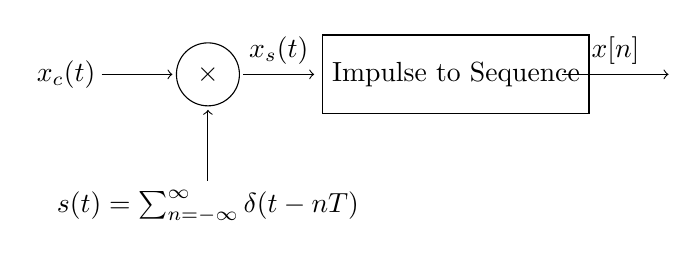
\begin{tikzpicture}[scale=0.9]
    \node at (-3,0) {$x_c(t)$};
    \draw[->] (-2.5,0) -- (-1.5,0);
    \node[draw, circle, minimum size=0.8cm] (mult) at (-1,0) {$\times$};
    \draw[->] (-0.5,0) -- (0.5,0) node[midway, above] {$x_s(t)$};
    \node[draw, minimum width=2.5cm, minimum height=1cm] (conv) at (2.5,0) {Impulse to Sequence};
    \draw[->] (4,0) -- (5.5,0) node[midway, above] {$x[n]$};
    
    \draw[->] (-1,-1.5) -- (-1,-0.5);
    \node[below] at (-1,-1.5) {$s(t) = \sum_{n=-\infty}^{\infty}\delta(t-nT)$};
\end{tikzpicture}
\end{center}

% \vspace{0.3cm}
\textbf{Impulse Train Modulation}:
\[
x_s(t) = x_c(t) \cdot s(t) = x_c(t) \sum_{n=-\infty}^{\infty}\delta(t-nT)
\]

% \vspace{0.3cm}
\textbf{Using Sifting Property} $x(t)\delta(t) = x(0)\delta(t)$:
\[
x_s(t) = \sum_{n=-\infty}^{\infty}x_c(nT)\delta(t-nT)
\]
\end{frame}

\begin{frame}{Time-Domain Visualization: Sampling Process}
\begin{center}
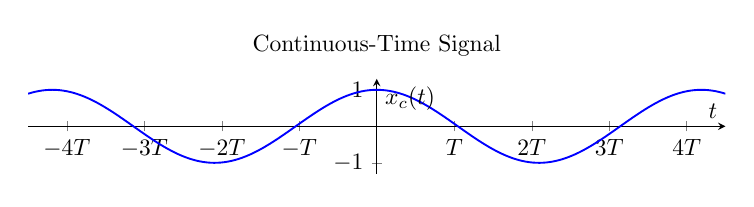
\begin{tikzpicture}[scale=0.85]
    % Original signal
    \begin{axis}[
        width=12cm, height=3cm,
        xlabel={$t$},
        ylabel={$x_c(t)$},
        xmin=-4.5, xmax=4.5,
        ymin=-1.3, ymax=1.3,
        samples=200,
        axis lines=middle,
        xtick={-4,-3,-2,-1,0,1,2,3,4},
        xticklabels={$-4T$,$-3T$,$-2T$,$-T$,$0$,$T$,$2T$,$3T$,$4T$},
        title={Continuous-Time Signal}
    ]
    \addplot[blue, thick, domain=-4.5:4.5] {cos(deg(1.5*x))};
    \end{axis}
\end{tikzpicture}
\end{center}

\begin{center}
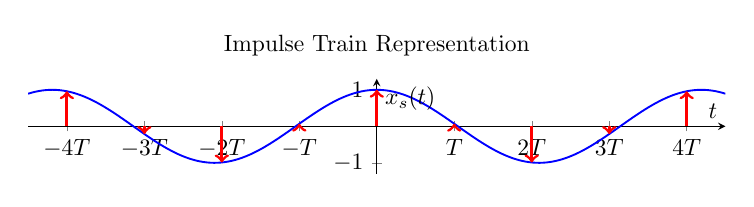
\begin{tikzpicture}[scale=0.85]
    % Sampled signal (impulse train)
    \begin{axis}[
        width=12cm, height=3cm,
        xlabel={$t$},
        ylabel={$x_s(t)$},
        xmin=-4.5, xmax=4.5,
        ymin=-1.3, ymax=1.3,
        axis lines=middle,
        xtick={-4,-3,-2,-1,0,1,2,3,4},
        xticklabels={$-4T$,$-3T$,$-2T$,$-T$,$0$,$T$,$2T$,$3T$,$4T$},
        title={Impulse Train Representation}
    ]
    \addplot[blue, thick, domain=-4.5:4.5, samples=200, forget plot] {cos(deg(1.5*x))};
    \foreach \n in {-4,-3,-2,-1,0,1,2,3,4} {
        \edef\temp{\noexpand\draw[->, red, very thick] (axis cs:\n,0) -- (axis cs:\n,{cos(deg(1.5*\n))});}
        \temp
    }
    \end{axis}
\end{tikzpicture}
\end{center}
\end{frame}

\begin{frame}{Time-Domain: Discrete-Time Sequence}
\begin{center}
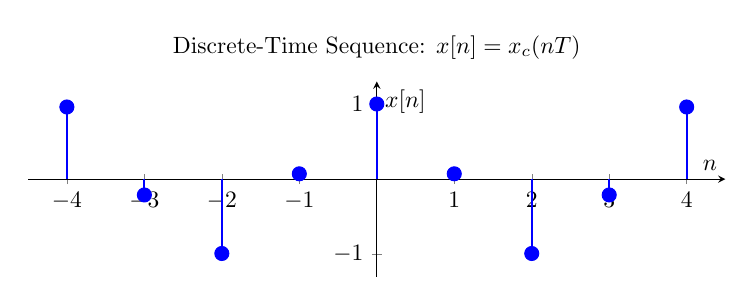
\begin{tikzpicture}[scale=0.85]
    \begin{axis}[
        width=12cm, height=4.5cm,
        xlabel={$n$},
        ylabel={$x[n]$},
        xmin=-4.5, xmax=4.5,
        ymin=-1.3, ymax=1.3,
        axis lines=middle,
        xtick={-4,-3,-2,-1,0,1,2,3,4},
        title={Discrete-Time Sequence: $x[n] = x_c(nT)$}
    ]
    % Sample points
    \addplot[only marks, blue, mark=*, mark size=3pt] coordinates {
        (-4,{cos(deg(-6))}) (-3,{cos(deg(-4.5))}) (-2,{cos(deg(-3))})
        (-1,{cos(deg(-1.5))}) (0,{cos(deg(0))}) (1,{cos(deg(1.5))})
        (2,{cos(deg(3))}) (3,{cos(deg(4.5))}) (4,{cos(deg(6))})
    };
    % Stems
    \draw[blue, thick] (axis cs:-4,0) -- (axis cs:-4,{cos(deg(-6))});
    \draw[blue, thick] (axis cs:-3,0) -- (axis cs:-3,{cos(deg(-4.5))});
    \draw[blue, thick] (axis cs:-2,0) -- (axis cs:-2,{cos(deg(-3))});
    \draw[blue, thick] (axis cs:-1,0) -- (axis cs:-1,{cos(deg(-1.5))});
    \draw[blue, thick] (axis cs:0,0) -- (axis cs:0,{cos(deg(0))});
    \draw[blue, thick] (axis cs:1,0) -- (axis cs:1,{cos(deg(1.5))});
    \draw[blue, thick] (axis cs:2,0) -- (axis cs:2,{cos(deg(3))});
    \draw[blue, thick] (axis cs:3,0) -- (axis cs:3,{cos(deg(4.5))});
    \draw[blue, thick] (axis cs:4,0) -- (axis cs:4,{cos(deg(6))});
    \end{axis}
\end{tikzpicture}
\end{center}

\textbf{Key Observation}: Time normalization
\begin{itemize}
    \item $x_s(t)$: Spacing = $T$ seconds
    \item $x[n]$: Spacing = 1 'sample index' (dimensionless)
    % \item Frequency axis will be normalized correspondingly
\end{itemize}
\end{frame}

\section{Frequency Domain}

\begin{frame}{Frequency-Domain: Fourier Transform of Impulse Train}
\textbf{Impulse Train in Time Domain}:
\[
s(t) = \sum_{n=-\infty}^{\infty}\delta(t-nT)
\]

\vspace{0.3cm}
\textbf{Fourier Transform (Impulse Train in Frequency)}:
\[
S(j\Omega) = \frac{2\pi}{T}\sum_{k=-\infty}^{\infty}\delta(\Omega - k\Omega_s), \quad \Omega_s = \frac{2\pi}{T}
\]

\begin{center}
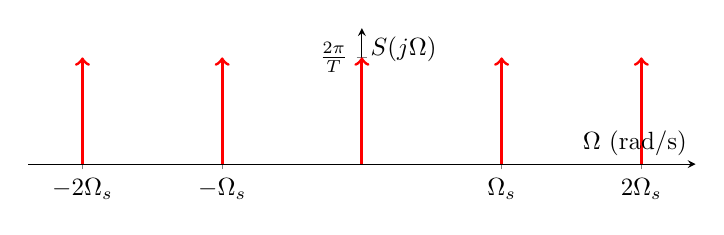
\begin{tikzpicture}[scale=0.9]
    \begin{axis}[
        width=11cm, height=3.5cm,
        xlabel={$\Omega$ (rad/s)},
        ylabel={$S(j\Omega)$},
        xmin=-15, xmax=15,
        ymin=0, ymax=8,
        axis lines=middle,
        xtick={-12.56,-6.28,0,6.28,12.56},
        xticklabels={$-2\Omega_s$,$-\Omega_s$,$0$,$\Omega_s$,$2\Omega_s$},
        ytick={6.28},
        yticklabels={$\frac{2\pi}{T}$}
    ]
    % Draw impulses
    \draw[->, red, very thick] (axis cs:-12.56,0) -- (axis cs:-12.56,6.28);
    \draw[->, red, very thick] (axis cs:-6.28,0) -- (axis cs:-6.28,6.28);
    \draw[->, red, very thick] (axis cs:0,0) -- (axis cs:0,6.28);
    \draw[->, red, very thick] (axis cs:6.28,0) -- (axis cs:6.28,6.28);
    \draw[->, red, very thick] (axis cs:12.56,0) -- (axis cs:12.56,6.28);
    \end{axis}
\end{tikzpicture}
\end{center}
\end{frame}

\begin{frame}{Frequency-Domain Representation of Sampling}
\textbf{Convolution Property}: $x_s(t) = x_c(t) \cdot s(t)$
\[
X_s(j\Omega) = \frac{1}{2\pi}X_c(j\Omega) * S(j\Omega)
\]

\vspace{0.3cm}
\textbf{Result - Periodic Replication}:
\[
\boxed{X_s(j\Omega) = \frac{1}{T}\sum_{k=-\infty}^{\infty}X_c(j(\Omega - k\Omega_s))}
\]

\vspace{0.3cm}
\textbf{Physical Interpretation}:
\begin{itemize}
    \item Original spectrum $X_c(j\Omega)$ is \textbf{replicated} at intervals of $\Omega_s$
    \item Scaled by factor $\frac{1}{T}$
    \item Copies centered at $\Omega = 0, \pm\Omega_s, \pm2\Omega_s, ...$
\end{itemize}
\end{frame}

\begin{frame}{Case 1: No Aliasing ($\Omega_s > 2\Omega_N$)}
\begin{center}
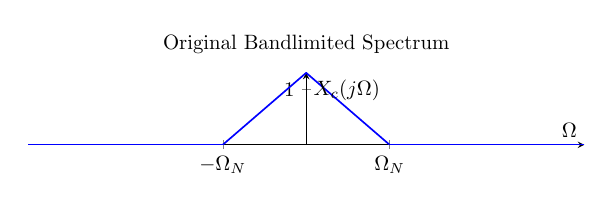
\begin{tikzpicture}[scale=0.75]
    % Original spectrum
    \begin{axis}[
        width=11cm, height=2.8cm,
        xlabel={$\Omega$},
        ylabel={$X_c(j\Omega)$},
        ylabel style={rotate=-90, anchor=south, xshift=1cm, yshift=0.5cm},
        xmin=-10, xmax=10,
        ymin=0, ymax=1.3,
        axis lines=middle,
        xtick={-3,3},
        xticklabels={$-\Omega_N$,$\Omega_N$},
        title={Original Bandlimited Spectrum},
        ytick={1},
        yticklabels={1}
    ]
    \addplot[blue, thick, domain=-3:3] {1.3*(1 - abs(x)/3)};
    \addplot[blue, thick, domain=-10:-3] {0};
    \addplot[blue, thick, domain=3:10] {0};
    \end{axis}
\end{tikzpicture}
\end{center}

\begin{center}
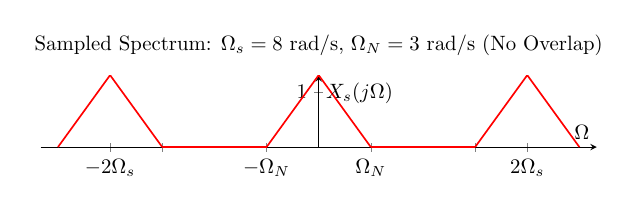
\begin{tikzpicture}[scale=0.75]
    % Sampled spectrum - no aliasing
    \begin{axis}[
        width=11cm, height=2.8cm,
        xlabel={$\Omega$},
        ylabel={$X_s(j\Omega)$},
        ylabel style={rotate=-90, anchor=south, xshift=1cm, yshift=0.5cm},
        xmin=-16, xmax=16,
        ymin=0, ymax=1.3,
        axis lines=middle,
        xtick={-12,-9,-3,0,3,9,12},
        xticklabels={$-2\Omega_s$,{},$-\Omega_N$,$0$,$\Omega_N$,{},$2\Omega_s$},
        title={Sampled Spectrum: $\Omega_s = 8$ rad/s, $\Omega_N = 3$ rad/s (No Overlap)},
        ytick={1},
        yticklabels={1}
    ]
    % Center copy
    \addplot[red, thick, domain=-3:3] {1.3*(1 - abs(x)/3)};
    % Left copy at -12
    \addplot[red, thick, domain=-15:-9] {1.3*(1 - abs(x+12)/3)};
    % Right copy at 12
    \addplot[red, thick, domain=9:15] {1.3*(1 - abs(x-12)/3)};
    % Zero elsewhere
    \addplot[red, thick, domain=-9:-3] {0};
    \addplot[red, thick, domain=3:9] {0};
    \end{axis}
\end{tikzpicture}
\end{center}
\end{frame}

\begin{frame}{Case 2: Aliasing ($\Omega_s < 2\Omega_N$)}
\begin{center}
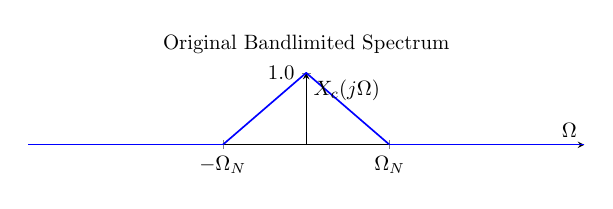
\begin{tikzpicture}[scale=0.75]
    % Original spectrum
    \begin{axis}[
        width=11cm, height=2.8cm,
        xlabel={$\Omega$},
        ylabel={$X_c(j\Omega)$},
        ylabel style={at={(axis cs:-9,0.85)}, anchor=center},
        xmin=-10, xmax=10,
        ymin=0, ymax=1.0,
        axis lines=middle,
        xtick={-3,3},
        xticklabels={$-\Omega_N$,$\Omega_N$},
        title={Original Bandlimited Spectrum},
        ytick={1.0},
        yticklabels={1.0}
    ]
    \addplot[blue, thick, domain=-3:3] {1.0*(1 - abs(x)/3)};
    \addplot[blue, thick, domain=-10:-3] {0};
    \addplot[blue, thick, domain=3:10] {0};
    \end{axis}
\end{tikzpicture}
\end{center}

\begin{center}
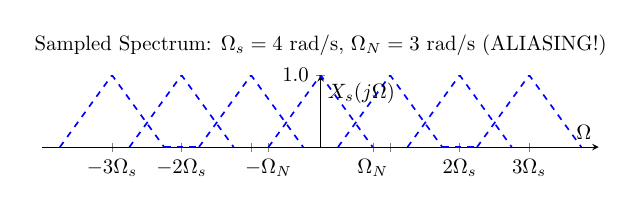
\begin{tikzpicture}[scale=0.75]
    % Sampled spectrum - aliasing
    \begin{axis}[
        width=11cm, height=2.8cm,
        xlabel={$\Omega$},
        ylabel={$X_s(j\Omega)$},
        ylabel style={at={(axis cs:-15,0.85)}, anchor=center},
        xmin=-16, xmax=16,
        ymin=0, ymax=1.0,
        axis lines=middle,
        xtick={-12,-8,-4,-3,0,3,4,8,12},
        xticklabels={$-3\Omega_s$,$-2\Omega_s$,{},$-\Omega_N$,$0$,$\Omega_N$,{},$2\Omega_s$,$3\Omega_s$},
        title={Sampled Spectrum: $\Omega_s = 4$ rad/s, $\Omega_N = 3$ rad/s (ALIASING!)},
        ytick={1.0},
        yticklabels={1.0}
    ]
    % Center copy at 0
    \addplot[blue, dashed, thick, domain=-3:3, samples=100] {1.0*(1 - abs(x)/3)};
    
    % Copies at ±4 (overlapping with center)
    \addplot[blue, dashed, thick, domain=-7:-1, samples=100] {1.0*(1 - abs(x+4)/3)};
    \addplot[blue, dashed, thick, domain=1:7, samples=100] {1.0*(1 - abs(x-4)/3)};
    
    % Copies at ±8
    \addplot[blue, dashed, thick, domain=-11:-5, samples=100] {1.0*(1 - abs(x+8)/3)};
    \addplot[blue, dashed, thick, domain=5:11, samples=100] {1.0*(1 - abs(x-8)/3)};
    
    % Copies at ±12
    \addplot[blue, dashed, thick, domain=-15:-9, samples=100] {1.0*(1 - abs(x+12)/3)};
    \addplot[blue, dashed, thick, domain=9:15, samples=100] {1.0*(1 - abs(x-12)/3)};
    
    % Zero elsewhere
    \addplot[blue, dashed, thick, domain=-9:-7] {0};
    \addplot[blue, dashed, thick, domain=7:9] {0};
    \end{axis}
\end{tikzpicture}
\end{center}
\end{frame}


\begin{frame}{Relation Between $X_s(j\Omega)$ and $X(e^{j\omega})$}
\textbf{From Impulse Train}:
\[
X_s(j\Omega) = \sum_{n=-\infty}^{\infty}x_c(nT)e^{-j\Omega nT}
\]

\textbf{DTFT of Sequence}:
\[
X(e^{j\omega}) = \sum_{n=-\infty}^{\infty}x[n]e^{-j\omega n}
\]

% \vspace{0.3cm}
\textbf{Relationship - Frequency Scaling}:
\[
\boxed{X(e^{j\omega}) = X_s(j\Omega)\Big|_{\Omega = \omega/T} = X_s(j\omega/T)}
\]

or equivalently:
\[
\boxed{X(e^{j\omega}) = \frac{1}{T}\sum_{k=-\infty}^{\infty}X_c\left(j\frac{\omega - 2\pi k}{T}\right)}
\]

\textbf{Normalization}: $\Omega = \Omega_s$ maps to $\omega = 2\pi$
\end{frame}

\begin{frame}{Frequency Axis Normalization}
\begin{center}
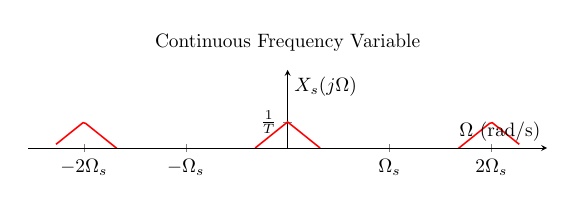
\begin{tikzpicture}[scale=0.7]
    % X_s(jOmega)
    \begin{axis}[
        width=11cm, height=3cm,
        xlabel={$\Omega$ (rad/s)},
        ylabel={$X_s(j\Omega)$},
        xmin=-16, xmax=16,
        ymin=0, ymax=1.0,
        axis lines=middle,
        xtick={-12.56,-6.28,0,6.28,12.56},
        xticklabels={$-2\Omega_s$,$-\Omega_s$,$0$,$\Omega_s$,$2\Omega_s$},
        title={Continuous Frequency Variable},
        ytick={0.333},
        yticklabels={$\frac{1}{T}$}
    ]
    \addplot[red, thick, domain=-2:2] {0.333*(1 - abs(x)/2)};
    \addplot[red, thick, domain=-14.28:-10.28] {0.333*(1 - abs(x+12.56)/2)};
    \addplot[red, thick, domain=10.28:14.28] {0.333*(1 - abs(x-12.56)/2)};
    \end{axis}
\end{tikzpicture}
\end{center}

\begin{center}
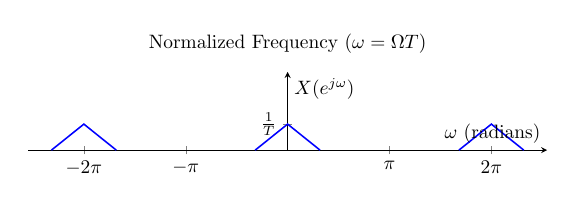
\begin{tikzpicture}[scale=0.7]
    % X(e^jw)
    \begin{axis}[
        width=11cm, height=3cm,
        xlabel={$\omega$ (radians)},
        ylabel={$X(e^{j\omega})$},
        xmin=-8, xmax=8,
        ymin=0, ymax=1.0,
        axis lines=middle,
        xtick={-6.28,-3.14,0,3.14,6.28},
        xticklabels={$-2\pi$,$-\pi$,$0$,$\pi$,$2\pi$},
        title={Normalized Frequency ($\omega = \Omega T$)},
        ytick={0.333},
        yticklabels={$\frac{1}{T}$}
    ]
    \addplot[blue, thick, domain=-1:1] {0.333*(1 - abs(x))};
    \addplot[blue, thick, domain=-7.28:-5.28] {0.333*(1 - abs(x+6.28))};
    \addplot[blue, thick, domain=5.28:7.28] {0.333*(1 - abs(x-6.28))};
    \end{axis}
\end{tikzpicture}
\end{center}

\textbf{Key Points}:
\begin{itemize}
    \item $\Omega_s = 2\pi/T$ maps to $\omega = 2\pi$
    \item $X(e^{j\omega})$ is always $2\pi$-periodic
\end{itemize}
\end{frame}

\section{Nyquist Theorem}

\begin{frame}{Nyquist-Shannon Sampling Theorem}
\textbf{Statement}:

Let $x_c(t)$ be a bandlimited signal with:
\[
X_c(j\Omega) = 0 \quad \text{for } |\Omega| \geq \Omega_N
\]

Then $x_c(t)$ is \textbf{uniquely determined} by its samples $x[n] = x_c(nT)$ if:
\[
\boxed{\Omega_s = \frac{2\pi}{T} \geq 2\Omega_N}
\]

\vspace{0.5cm}
\textbf{Terminology}:
\begin{itemize}
    \item $\Omega_N$ = \textbf{Nyquist frequency} (highest frequency in signal)
    \item $2\Omega_N$ = \textbf{Nyquist rate} (minimum sampling frequency)
    \item $\Omega_s/2$ = \textbf{Folding frequency}
\end{itemize}
\end{frame}

\begin{frame}{Reconstruction from Samples}
\textbf{System}:
\begin{center}
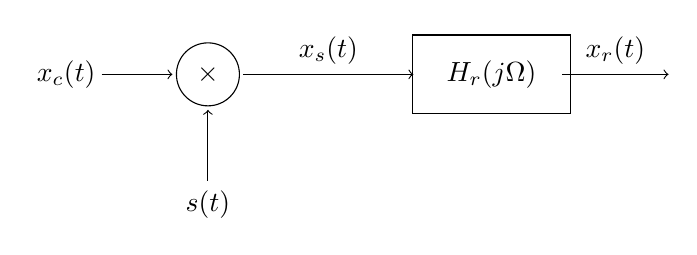
\begin{tikzpicture}[scale=0.9]
    \node at (-4.5,0) {$x_c(t)$};
    \draw[->] (-4,0) -- (-3,0);
    \node[draw, circle, minimum size=0.8cm] (mult) at (-2.5,0) {$\times$};
    \draw[->] (-2,0) -- (0.4,0) node[midway, above] {$x_s(t)$};
    \node[draw, minimum width=2cm, minimum height=1cm] (filt) at (1.5,0) {$H_r(j\Omega)$};
    \draw[->] (2.5,0) -- (4,0) node[midway, above] {$x_r(t)$};
    
    \draw[->] (-2.5,-1.5) -- (-2.5,-0.5);
    \node[below] at (-2.5,-1.5) {$s(t)$};
\end{tikzpicture}
\end{center}

\vspace{0.3cm}
\textbf{Ideal Reconstruction Filter}:
\[
H_r(j\Omega) = \begin{cases}
T, & |\Omega| \leq \Omega_c \\
0, & |\Omega| > \Omega_c
\end{cases}
\]

where $\Omega_N \leq \Omega_c \leq (\Omega_s - \Omega_N)$

\vspace{0.3cm}
\textbf{Output}:
\[
X_r(j\Omega) = H_r(j\Omega) \cdot X_s(j\Omega) = X_c(j\Omega) \quad \text{if } \Omega_s \geq 2\Omega_N
\]
\end{frame}

\begin{frame}{Ideal Lowpass Reconstruction Filter}
\begin{center}
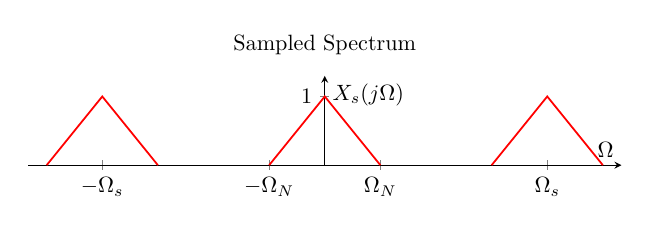
\begin{tikzpicture}[scale=0.8]
    % Sampled spectrum
    \begin{axis}[
        width=11cm, height=3cm,
        xlabel={$\Omega$},
        ylabel={$X_s(j\Omega)$},
        ylabel style={at={(axis cs:-15,0.65)}, anchor=center},
        xmin=-16, xmax=16,
        ymin=0, ymax=1.3,
        axis lines=middle,
        xtick={-12,-3,0,3,12},
        xticklabels={$-\Omega_s$,$-\Omega_N$,$0$,$\Omega_N$,$\Omega_s$},
        ytick={1},
        yticklabels={1},
        title={Sampled Spectrum}
    ]
    \addplot[red, thick, domain=-3:3] {1*(1 - abs(x)/3)};
    \addplot[red, thick, domain=-15:-9] {1*(1 - abs(x+12)/3)};
    \addplot[red, thick, domain=9:15] {1*(1 - abs(x-12)/3)};
    \end{axis}
\end{tikzpicture}
\end{center}

\begin{center}
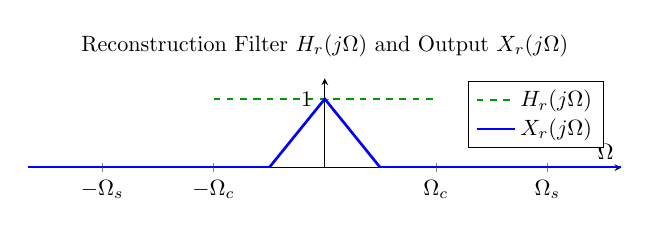
\begin{tikzpicture}[scale=0.8]
    % Filter response and output
    \begin{axis}[
        width=11cm, height=3cm,
        xlabel={$\Omega$},
        ylabel={},
        xmin=-16, xmax=16,
        ymin=0, ymax=1.3,
        axis lines=middle,
        xtick={-12,-6,0,6,12},
        xticklabels={$-\Omega_s$,$-\Omega_c$,$0$,$\Omega_c$,$\Omega_s$},
        ytick={1},
        yticklabels={1},
        title={Reconstruction Filter $H_r(j\Omega)$ and Output $X_r(j\Omega)$},
        legend pos=north east
    ]
    % Filter
    \addplot[green!60!black, dashed, thick, domain=-6:6] {1};
    \addlegendentry{$H_r(j\Omega)$}
    \addplot[green!60!black, dashed, thick, domain=-16:-6, forget plot] {0};
    \addplot[green!60!black, dashed, thick, domain=6:16, forget plot] {0};
    % Output (scaled by T)
    \addplot[blue, very thick, domain=-3:3] {1*(1 - abs(x)/3)};
    \addlegendentry{$X_r(j\Omega)$}
    \addplot[blue, very thick, domain=-16:-3, forget plot] {0};
    \addplot[blue, very thick, domain=3:16, forget plot] {0};
    \end{axis}
\end{tikzpicture}
\end{center}

\textbf{Result}: $X_r(j\Omega) = X_c(j\Omega)$ $\Rightarrow$ $x_r(t) = x_c(t)$
\end{frame}

\section{Examples}

\begin{frame}{Example 1: Sampling a Sinusoid (No Aliasing)}
\textbf{Signal}: $x_c(t) = \cos(\Omega_0 t)$ with $\Omega_0 = 4000\pi$ rad/s

\textbf{Sampling}: $T = 1/6000$ s $\Rightarrow$ $\Omega_s = 12000\pi$ rad/s

\vspace{0.3cm}
\textbf{Check Nyquist}: $\Omega_s = 12000\pi > 2\Omega_0 = 8000\pi$ \checkmark

\vspace{0.3cm}
\textbf{Sampled Sequence}:
\[
x[n] = \cos(4000\pi \cdot n/6000) = \cos(2\pi n/3)
\]

Normalized frequency: $\omega_0 = \Omega_0, T = 2\pi/3$

\vspace{0.3cm}
\textbf{Fourier Transform}:
\[
X_c(j\Omega) = \pi\delta(\Omega - 4000\pi) + \pi\delta(\Omega + 4000\pi)
\]

\textbf{After Sampling}:
\[
X(e^{j\omega}) = \pi\delta(\omega - 2\pi/3) + \pi\delta(\omega + 2\pi/3) + \text{periodic}
\]
\end{frame}


\begin{frame}{Example 1: Frequency Domain Visualization}
\begin{center}
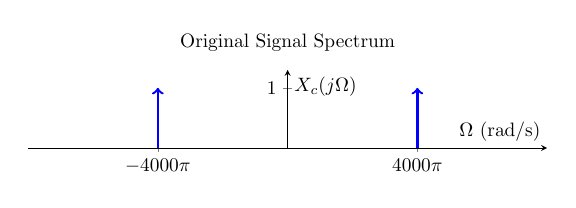
\begin{tikzpicture}[scale=0.7]
    \begin{axis}[
        width=11cm, height=3cm,
        xlabel={$\Omega$ (rad/s)},
        ylabel={$X_c(j\Omega)$},
        ylabel style={at={(axis cs:-7500,0.65)}, anchor=center},
        xmin=-8000, xmax=8000,
        ymin=0, ymax=1.3,
        axis lines=middle,
        xtick={-4000,0,4000},
        xticklabels={$-4000\pi$,$0$,$4000\pi$},
        ytick={1},
        yticklabels={1},
        title={Original Signal Spectrum}
    ]
    \draw[->, blue, very thick] (axis cs:-4000,0) -- (axis cs:-4000,1);
    \draw[->, blue, very thick] (axis cs:4000,0) -- (axis cs:4000,1);
    \end{axis}
\end{tikzpicture}
\end{center}

\begin{center}
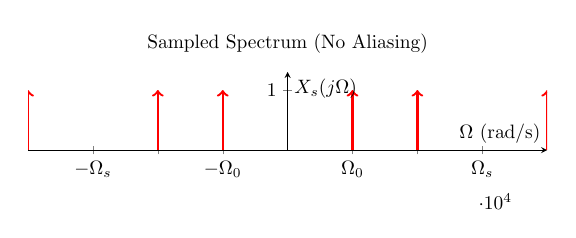
\begin{tikzpicture}[scale=0.7]
    \begin{axis}[
        width=11cm, height=3cm,
        xlabel={$\Omega$ (rad/s)},
        ylabel={$X_s(j\Omega)$},
        ylabel style={at={(axis cs:-15000,0.65)}, anchor=center},
        xmin=-16000, xmax=16000,
        ymin=0, ymax=1.3,
        axis lines=middle,
        xtick={-12000,-8000,-4000,0,4000,8000,12000},
        xticklabels={$-\Omega_s$,{},$-\Omega_0$,$0$,$\Omega_0$,{},$\Omega_s$},
        ytick={1},
        yticklabels={1},
        title={Sampled Spectrum (No Aliasing)}
    ]
    % Center
    \draw[->, red, very thick] (axis cs:-4000,0) -- (axis cs:-4000,1);
    \draw[->, red, very thick] (axis cs:4000,0) -- (axis cs:4000,1);
    % Left
    \draw[->, red, very thick] (axis cs:-16000,0) -- (axis cs:-16000,1);
    \draw[->, red, very thick] (axis cs:-8000,0) -- (axis cs:-8000,1);
    % Right
    \draw[->, red, very thick] (axis cs:8000,0) -- (axis cs:8000,1);
    \draw[->, red, very thick] (axis cs:16000,0) -- (axis cs:16000,1);
    \end{axis}
\end{tikzpicture}
\end{center}

\textbf{Reconstruction}: Lowpass filter extracts center copy → $x_r(t) = x_c(t)$
\end{frame}

\begin{frame}{Example 2: Sampling a Sinusoid (With Aliasing)}
\textbf{Signal}: $x_c(t) = \cos(\Omega_0 t)$ with $\Omega_0 = 16000\pi$ rad/s

\textbf{Sampling}: $T = 1/6000$ s $\Rightarrow$ $\Omega_s = 12000\pi$ rad/s

\vspace{0.3cm}
\textbf{Check Nyquist}: $\Omega_s = 12000\pi < 2\Omega_0 = 32000\pi$ \textcolor{red}{$\times$}

\vspace{0.3cm}
\textbf{Sampled Sequence}:
\[
x[n] = \cos(16000\pi \cdot n/6000) = \cos(8\pi n/3)
\]

But $\cos(8\pi n/3) = \cos(8\pi n/3 - 2\pi n) = \cos(2\pi n/3)$

\vspace{0.3cm}
\textbf{Same samples as Example 1!}

\textbf{Alias frequency}: $\Omega_{\text{alias}} = \Omega_s - \Omega_0 = 12000\pi - 16000\pi = -4000\pi$

Or equivalently: $|\Omega_{\text{alias}}| = 4000\pi$
\end{frame}

\begin{frame}{Example 2: Aliasing Visualization}
\begin{center}
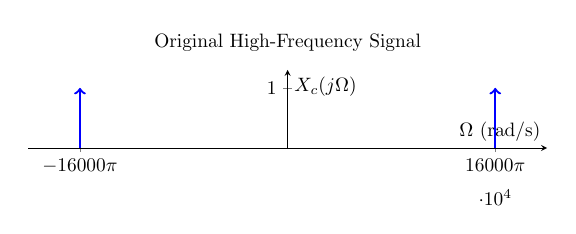
\begin{tikzpicture}[scale=0.7]
    \begin{axis}[
        width=11cm, height=3cm,
        xlabel={$\Omega$ (rad/s)},
        ylabel={$X_c(j\Omega)$},
        ylabel style={at={(axis cs:-18500,0.65)}, anchor=center},
        xmin=-20000, xmax=20000,
        ymin=0, ymax=1.3,
        axis lines=middle,
        xtick={-16000,0,16000},
        xticklabels={$-16000\pi$,$0$,$16000\pi$},
        ytick={1},
        yticklabels={1},
        title={Original High-Frequency Signal}
    ]
    \draw[->, blue, very thick] (axis cs:-16000,0) -- (axis cs:-16000,1);
    \draw[->, blue, very thick] (axis cs:16000,0) -- (axis cs:16000,1);
    \end{axis}
\end{tikzpicture}
\end{center}

\begin{center}
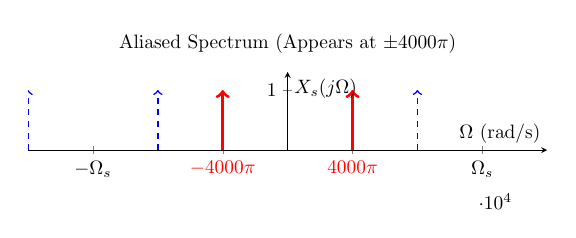
\begin{tikzpicture}[scale=0.7]
    \begin{axis}[
        width=11cm, height=3cm,
        xlabel={$\Omega$ (rad/s)},
        ylabel={$X_s(j\Omega)$},
        ylabel style={at={(axis cs:-15000,0.65)}, anchor=center},
        xmin=-16000, xmax=16000,
        ymin=0, ymax=1.3,
        axis lines=middle,
        xtick={-12000,-4000,0,4000,12000},
        xticklabels={$-\Omega_s$,{\color{red}$-4000\pi$},$0$,{\color{red}$4000\pi$},$\Omega_s$},
        ytick={1},
        yticklabels={1},
        title={Aliased Spectrum (Appears at $\pm 4000\pi$)}
    ]
    % Aliases appear at ±4000
    \draw[->, red, ultra thick] (axis cs:-4000,0) -- (axis cs:-4000,1);
    \draw[->, red, ultra thick] (axis cs:4000,0) -- (axis cs:4000,1);
    % Also at ±16000 (from adjacent periods)
    \draw[->, blue, dashed, thick] (axis cs:-16000,0) -- (axis cs:-16000,1);
    % At -8000 (from 16000 - 24000)
    \draw[->, blue, dashed, thick] (axis cs:-8000,0) -- (axis cs:-8000,1);
    % At 8000 (from -16000 + 24000)
    \draw[->, blue, dashed, thick] (axis cs:8000,0) -- (axis cs:8000,1);
    % Annotation
    % \node[red] at (axis cs:0,1.15) {Aliasing!};
    \end{axis}
\end{tikzpicture}
\end{center}

\textbf{Reconstruction}: Filter extracts $4000\pi$ → $x_r(t) = \cos(4000\pi t) \neq x_c(t)$
\end{frame}

\begin{frame}{Aliasing: Multiple Signals → Same Samples}
\textbf{Key Insight}: For any integer $k$:
\[
\cos[(\Omega_s k + \Omega_0)nT] = \cos(\Omega_0 nT)
\]

\vspace{0.3cm}
\textbf{Family of Alias Frequencies}:
\[
\Omega_{\text{alias}, k} = \Omega_0 + k\Omega_s, \quad k = 0, \pm 1, \pm 2, ...
\]

All produce the same sequence when sampled at rate $\Omega_s$!

\vspace{0.3cm}
\textbf{Example}: $\Omega_s = 12000\pi$, sample values $x[n] = \cos(2\pi n/3)$

\begin{center}
\begin{tabular}{|c|c|}
\hline
Frequency $\Omega_0$ (rad/s) & Normalized $\omega_0$ \\
\hline
$4000\pi$ & $2\pi/3$ \\
$16000\pi$ & $8\pi/3 = 2\pi/3 + 2\pi$ \\
$-8000\pi$ & $-4\pi/3 = 2\pi/3 - 2\pi$ \\
$28000\pi$ & $14\pi/3 = 2\pi/3 + 4\pi$ \\
\hline
\end{tabular}
\end{center}

\textbf{Resolution}: Restrict to $|\Omega_0| \leq \Omega_s/2$ (Nyquist criterion)
\end{frame}

\begin{frame}{Summary: Sampling in Frequency Domain}
\textbf{Key Equation}:
\[
X_s(j\Omega) = \frac{1}{T}\sum_{k=-\infty}^{\infty}X_c(j(\Omega - k\Omega_s))
\]

\vspace{0.3cm}
\textbf{Three Cases}:

\begin{enumerate}
    \item \textbf{$\Omega_s > 2\Omega_N$}: No overlap → Perfect reconstruction possible
    \item \textbf{$\Omega_s = 2\Omega_N$}: Critical sampling (Nyquist rate)
    \item \textbf{$\Omega_s < 2\Omega_N$}: Aliasing → Information loss
\end{enumerate}

\vspace{0.3cm}
\textbf{Practical Considerations}:
\begin{itemize}
    \item Real signals are never perfectly bandlimited
    \item Anti-aliasing filters used before sampling
    \item Oversampling provides guard band
    \item Trade-off: sampling rate vs. computation/storage
\end{itemize}
\end{frame}

\begin{frame}{Reconstruction Formula (Time Domain)}
\textbf{Ideal Lowpass Filter Impulse Response}:
\[
h_r(t) = \frac{\sin(\Omega_c t)}{\pi t}
\]

\vspace{0.3cm}
\textbf{Reconstruction Formula}:
\[
x_r(t) = \sum_{n=-\infty}^{\infty}x[n] h_r(t - nT) = \sum_{n=-\infty}^{\infty}x_c(nT)\frac{\sin[\Omega_c(t-nT)]}{\pi(t-nT)}
\]

For $\Omega_c = \pi/T$:
\[
\boxed{x_c(t) = \sum_{n=-\infty}^{\infty}x_c(nT)\frac{\sin[\pi(t-nT)/T]}{\pi(t-nT)/T}}
\]

\vspace{0.3cm}
\textbf{Interpolation}: Each sample weighted by sinc function

\textbf{Shannon Interpolation Formula}: Exact for bandlimited signals
\end{frame}

\begin{frame}{Conclusion}
\textbf{Main Results}:
\begin{enumerate}
    \item Sampling creates \textbf{periodic replication} in frequency domain
    \item \textbf{Nyquist criterion}: $\Omega_s \geq 2\Omega_N$ prevents aliasing
    \item \textbf{Perfect reconstruction} possible if Nyquist satisfied
    \item Frequency normalization: $\omega = \Omega T$
\end{enumerate}

\vspace{0.5cm}
\textbf{Practical Applications}:
\begin{itemize}
    \item Digital audio: $f_s = 44.1$ kHz (covers 0-20 kHz hearing range)
    \item Speech: $f_s = 8$ kHz (telephone quality)
    \item Video: Various rates depending on bandwidth
    \item Software-defined radio, data acquisition, control systems
\end{itemize}

\vspace{0.5cm}
\textbf{Next Topics}:
\begin{itemize}
    \item Practical A/D conversion, quantization effects
    \item Multirate signal processing, decimation, interpolation
    \item Filter design for anti-aliasing
\end{itemize}
\end{frame}

\end{document}